\section{SimTech}
\label{fundamentals:simtech}

Since 2005, the German federal and state government have been running the Excellence Initiative\footnote{\url{http://www.dfg.de/en/research_funding/programmes/excellence_initiative/index.html}}, which aims to promote cutting-edge research, thereby increasing the quality and international competitiveness of German universities.
In three rounds of funding, universities have competed with project proposals in three areas: Institutional Strategies, Graduate Schools, and Clusters of Excellence.
\nom{Simulation Technology}{SimTech} is one of the Clusters of Excellence that are funded by the Excellence Initiative.
In a partnership between the University of Stuttgart, the German Aerospace Center, the Fraunhofer Institute for Manufacturing Engineering and Automation, and the Max Planck Institute for Intelligent Systems, it combines over 60 projects from researchers in Engineering, Natural Science, and the Life and Social Sciences.
The aim of SimTech is to improve existing simulation strategies and to create new simulation solutions~\autocite{excellence:glance}.

In the SimTech project, seven individual research areas collaborate in seven different project networks, one of which is project network 6: \textit{Cyber Infrastructure and Beyond}\footnote{\url{http://www.simtech.uni-stuttgart.de/forschung/pn/PN6/index.en.html}}.
The goal of this project network is to build an easy-to-use infrastructure that supports scientists in their day to day work with simulations.

\subsection{SimTech SWfMS}

As part of this project, the SimTech SWfMS was developed.
It is a system that enables scientists to easily create, manage and execute simulation workflows which are a subcategory of scientific workflows~\autocite{workflow:simulation:flexibility}.
The SimTech SWfMS introduces extensions to the BPEL language that add functionality to support the requirements of simulation workflows, such as passing data by reference to support larger amounts of data often found in science~\autocite[also~see][]{workflow:simulation:modelling:datareferences}, or shared context between workflows~\autocite{workflow:simulation:modelling}.
Other extension introduces by the SimTech SWfMS to support simulation workflows include a service bus that supports late binding, rebinding, and legacy simulation software, as well as the \nom{Simulation Data Management System}{SIMPL} that provides unified access methods for arbitrary external data~\autocite{workflow:simulation:runtime}.
Additionally, extension where also made in the areas of flexibility to support a "model as you go" approach and in human user involvement to support human tasks for decision making, data manipulation, or workflow repair~\autocites{workflow:simulation:flexibility}{workflow:simulation:humanusers}.

The SimTech SWfMS consists of the \nom{SimTech Workflow Modeling \& Monitoring Tool}{SimTech Modeler} and the workflow middleware.
The SimTech Modeler is based on Eclipse JEE\footnote{\url{http://www.eclipse.org/ide/}} and extends its functionality with various plugins.
\autoref{image:modeler} shows the SimTech Modeler user interface.
It allows the user to create simulation workflows using a graph as visual representation, where vertices represent simulation tasks and edges describe the progression between those tasks.

\begin{figure}[!htbp]
	\centering
	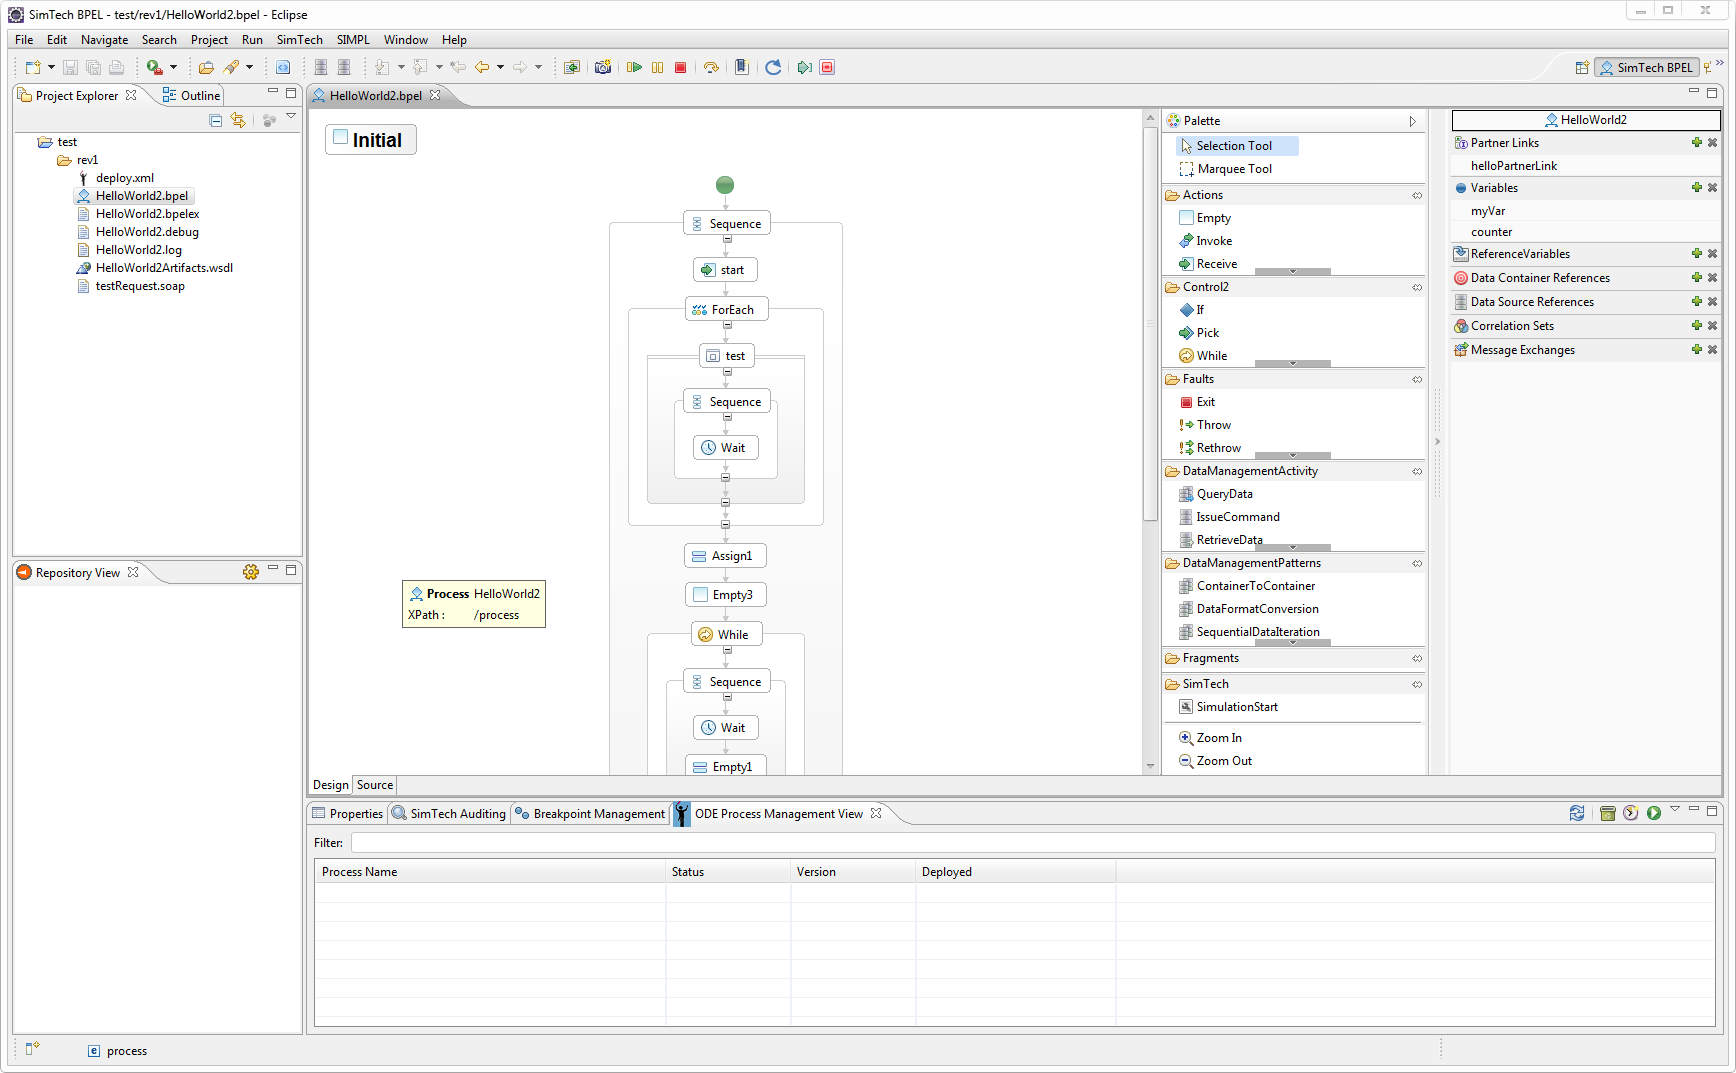
\includegraphics[width=\textwidth,interpolate=false]{fundamentals/assets/simtech_modeler}
	\caption{The SimTech Modeler user interface.}
	\label{image:modeler}
\end{figure}

Once the user is done modeling the simulation workflow, they click on a button to execute the workflow on the workflow middleware.
The middleware consists of various components, some of which are shown in \autoref{image:swfms}.
Most of them are executed by an application server, in this case Apache Tomcat\footnote{\url{http://tomcat.apache.org/}}.
The workflow is deployed on the workflow engine, in this case \nom{ODE Pluggable Framework}{ODE-PGF}\footnote{\url{http://www.iaas.uni-stuttgart.de/forschung/projects/ODE-PGF/}}, which executes the workflow step by step.
If a step involves the execution of a service, the ESB (Apache Service Mix\footnote{\url{http://servicemix.apache.org/}}) is called, which resolves the services and passes along the request and the response.
Further components include SimTech Auditing, which is used for auditing purposes.
It is connected to the workflow engine via a messaging middleware (Apache ActiveMQ\footnote{\url{http://activemq.apache.org/}}).
It is also connected to a database where it stores its data.

\begin{figure}[!htbp]
	\centering
	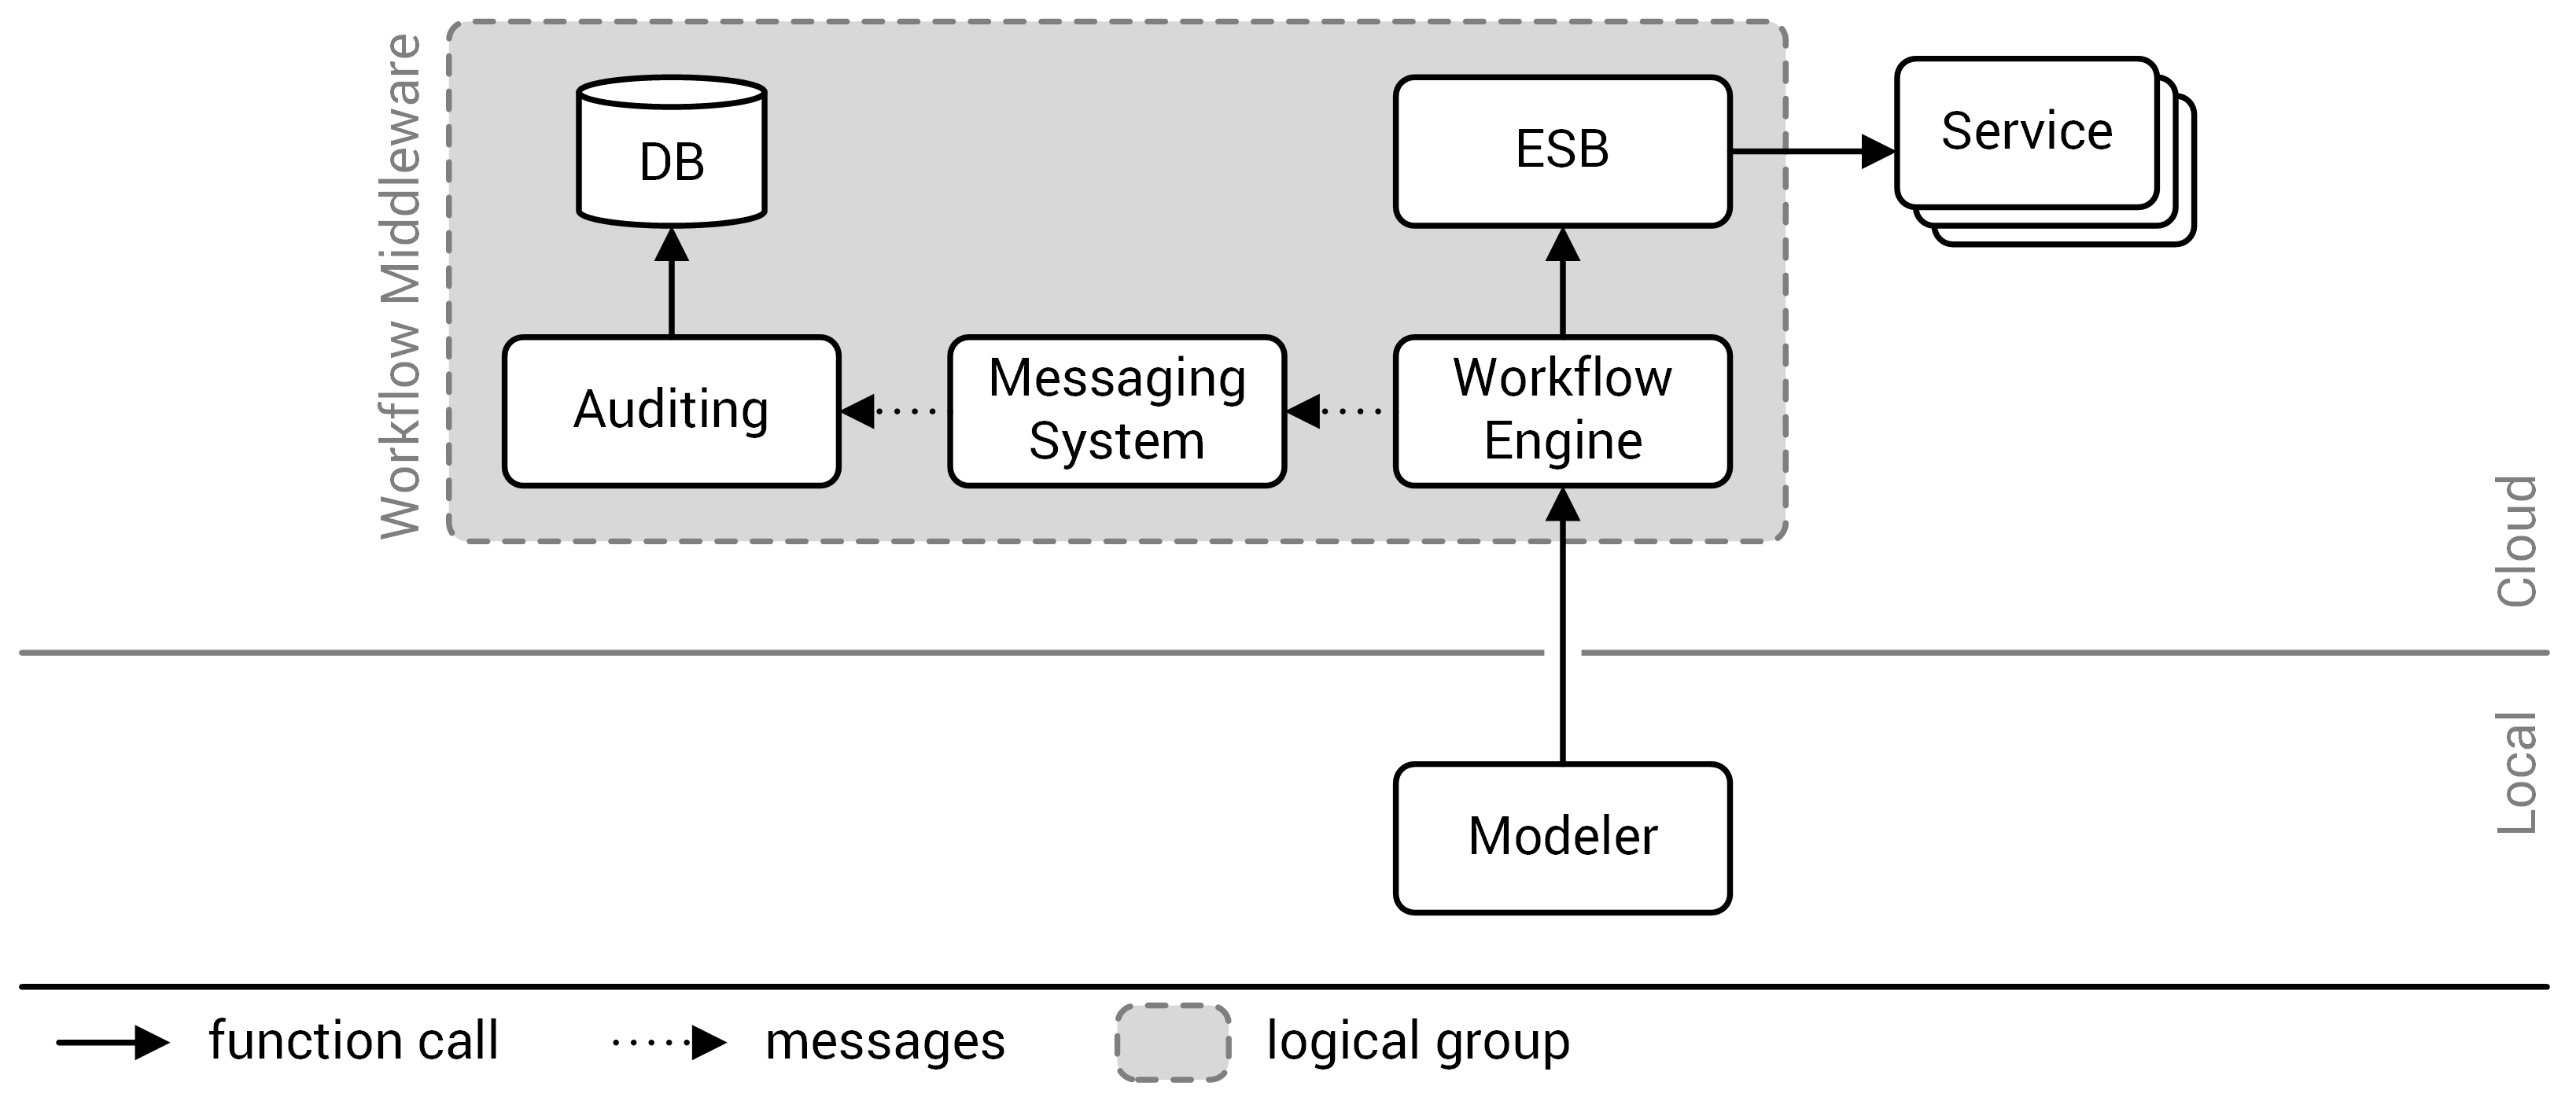
\includegraphics[width=\textwidth,interpolate=false]{fundamentals/assets/unmodified_architecture}
	\caption{Some of the SimTech SWfMS components.}
	\label{image:swfms}
\end{figure}
